\chapter{Other Measurement Data}

\section {Participant 1}
\begin{figure}[H]
  \centering
    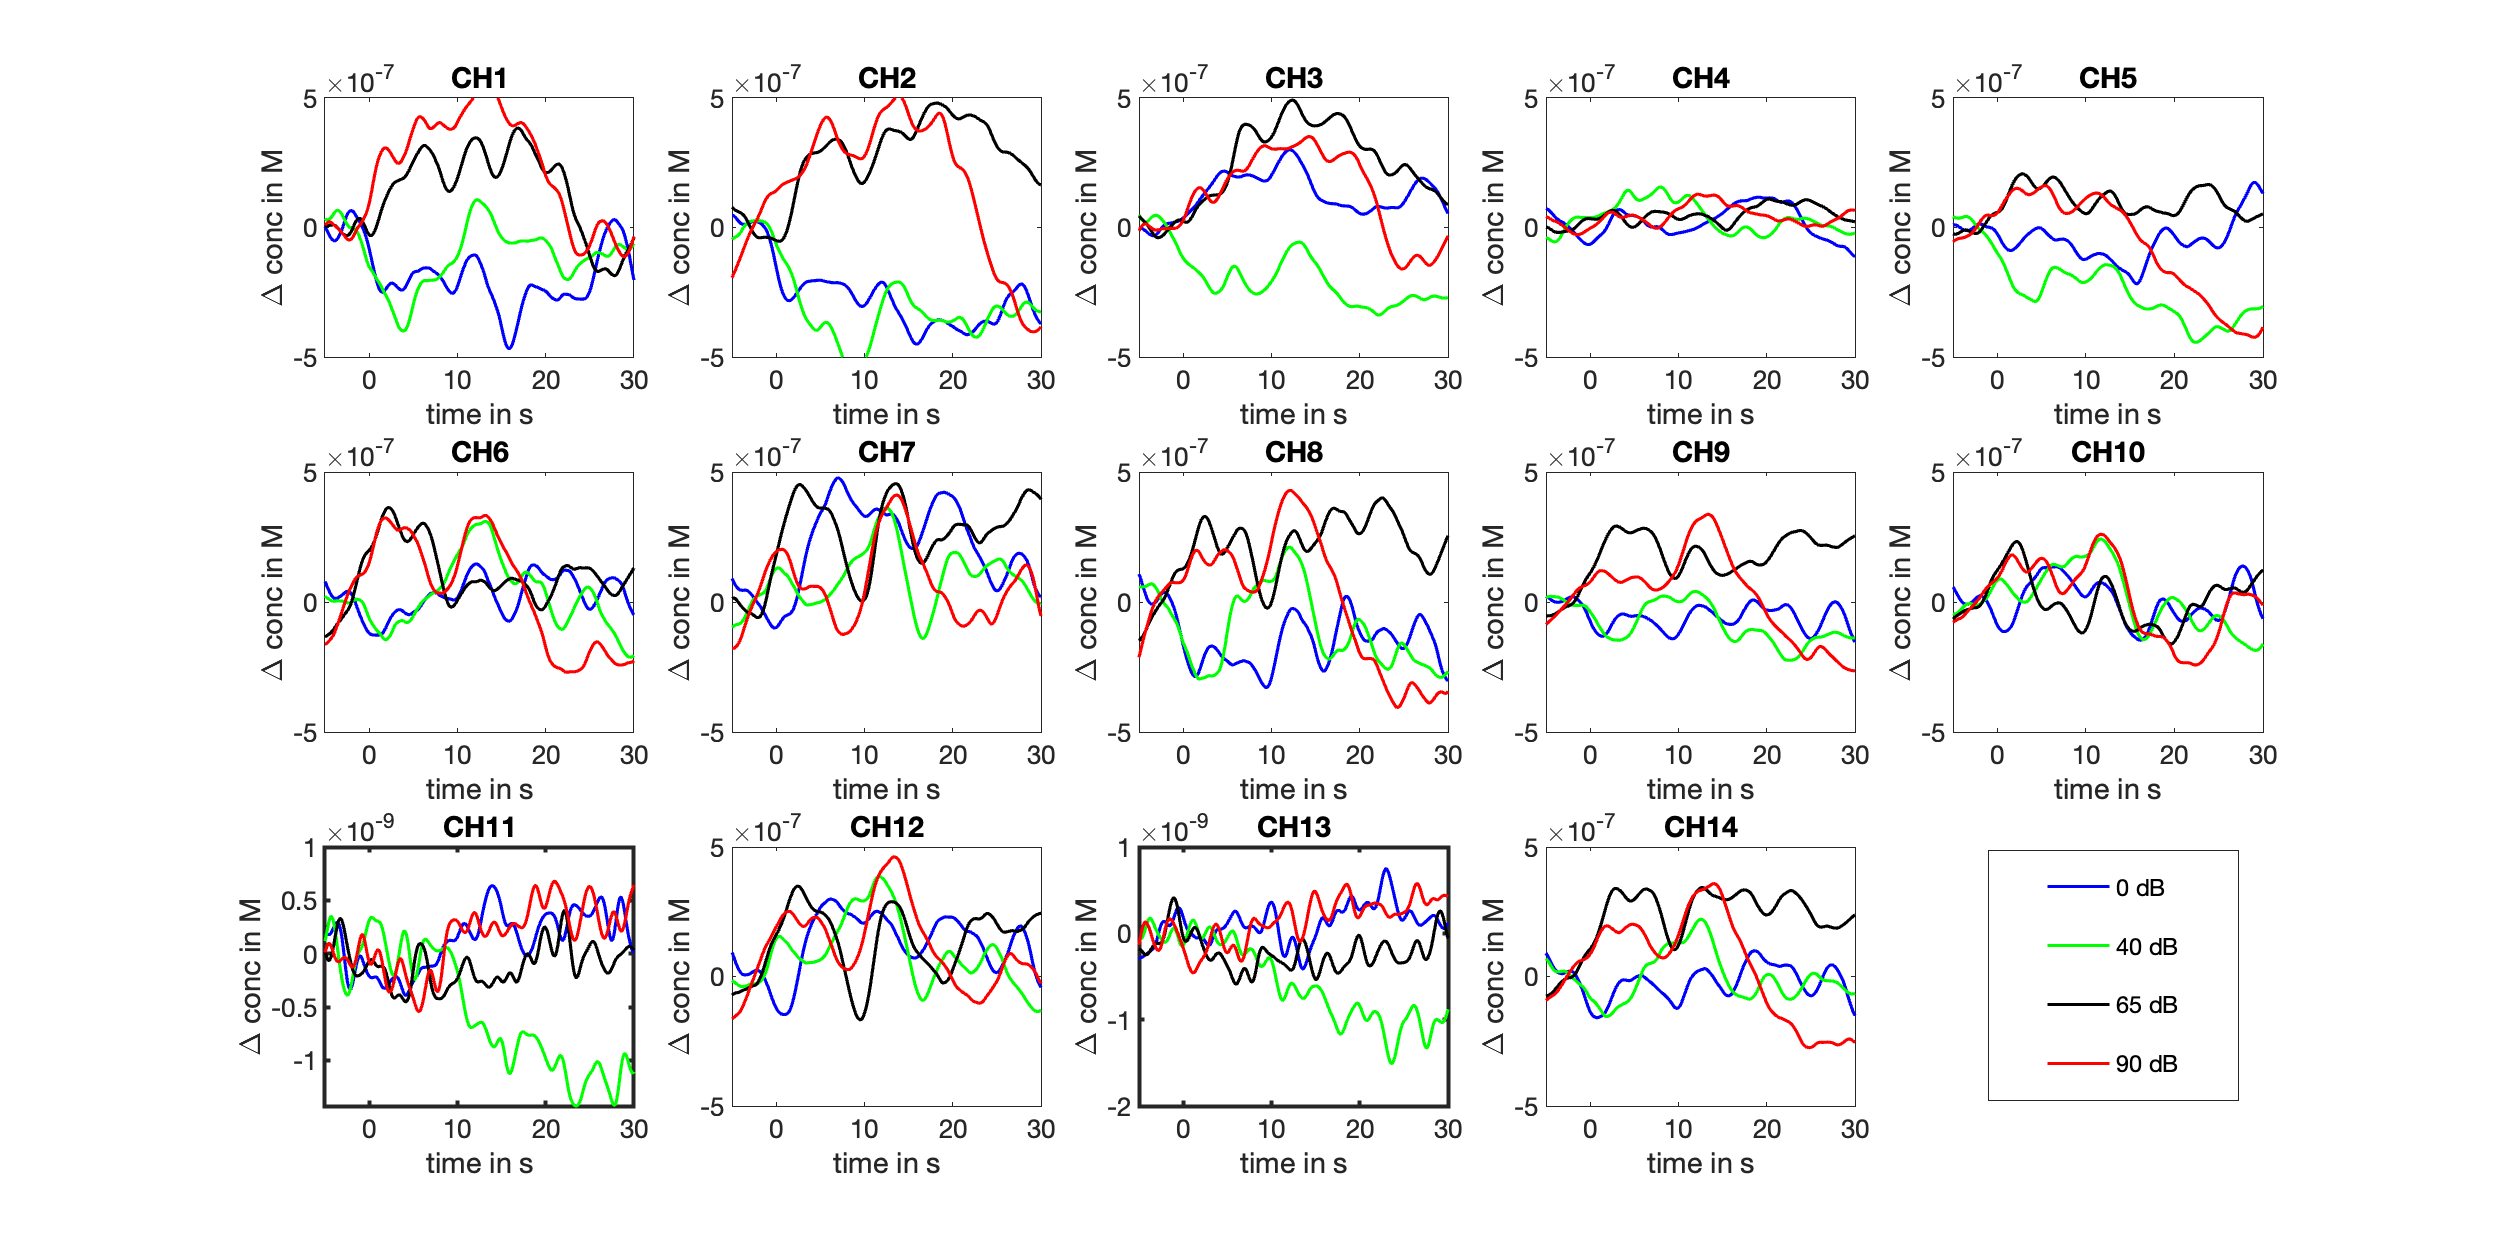
\includegraphics[scale=.4]{bilder/HbO_Mole/sub_chang_s_HbO.png}
  \caption{HbO measurement from participant 1.}
  \label{fig:somesignal}
  \medskip
  \footnotesize {Lines represent the block-averaged results over eight epochs. The averaged change of HbO concentration (in Mole) is plotted from 5 seconds before the start of the auditory stimuli to 30 seconds after the start of the stimuli. Four colours are used to differentiate the response from sound stimuli of different intensity levels.}
\end{figure}

\newpage

\begin{figure}[H]
  \centering
    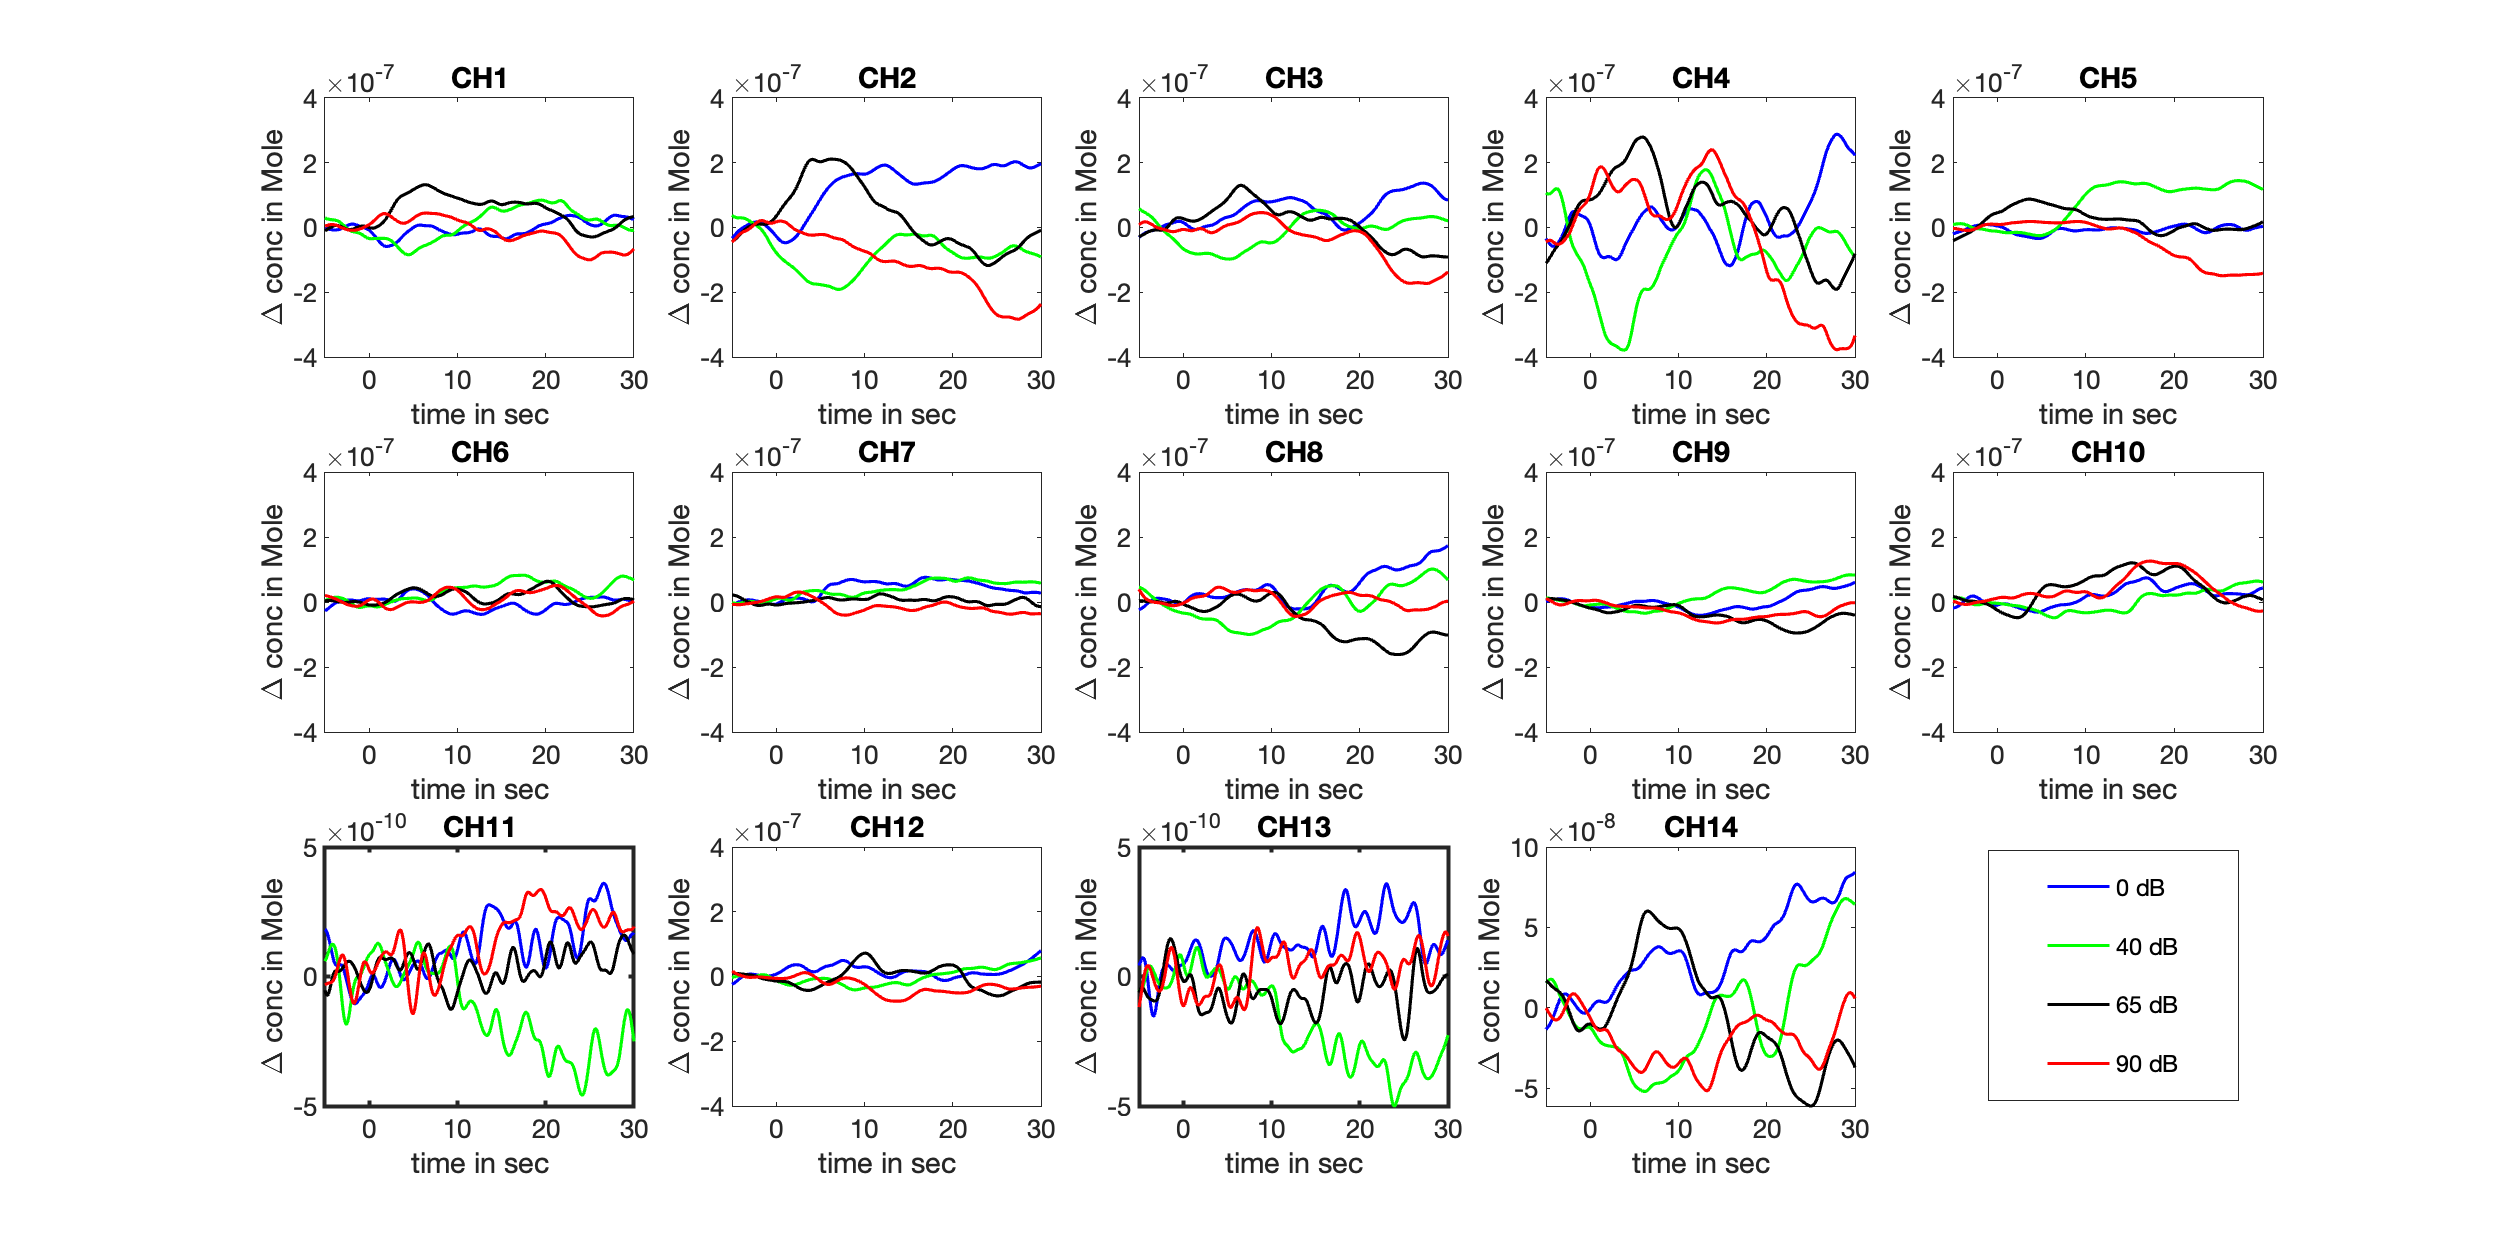
\includegraphics[scale=.4]{bilder/HbR_Mole/sub_chang_s_HbR.png}
  \caption{HbR measurement from participant 1.}
  \label{fig:somesignal}
  \medskip
  \footnotesize {Lines represent the block-averaged results over eight epochs. The averaged change of HbR concentration (in Mole) is plotted from 5 seconds before the start of the auditory stimuli to 30 seconds after the start of the stimuli. Four colours are used to differentiate the response from sound stimuli of different intensity levels.}
\end{figure}

\begin{figure}[H]
  \centering
    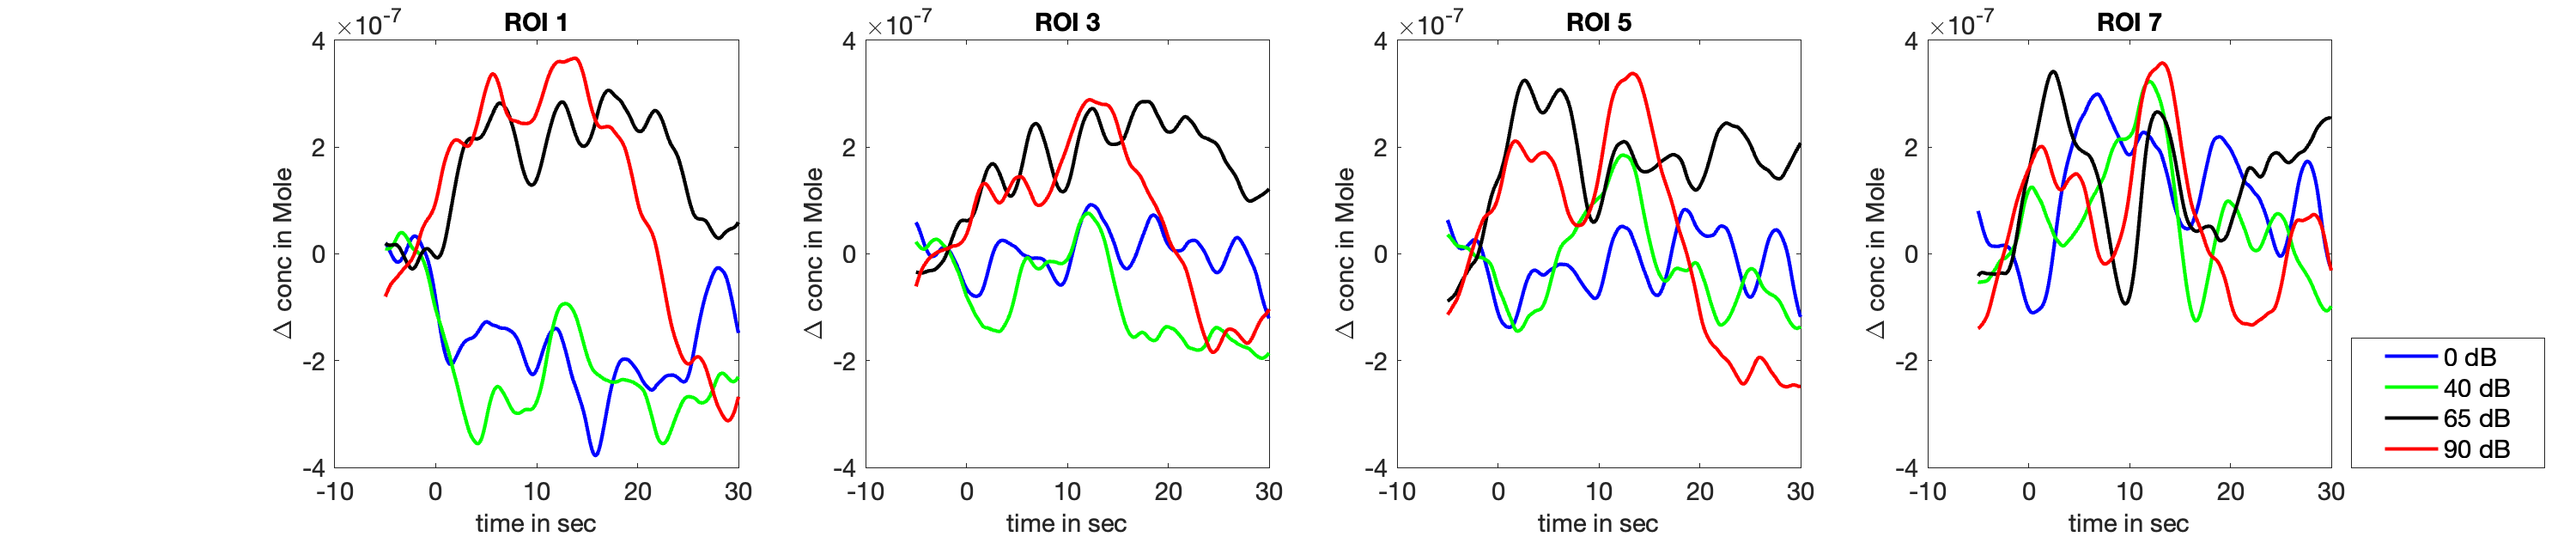
\includegraphics[scale=.29]{bilder/ROI/sub_chang_s_HbO.png}
  \caption{ROI measurement from participant 1.}
\end{figure}
\newpage


\section {Participant 2}

\begin{figure}[H]
  \centering
    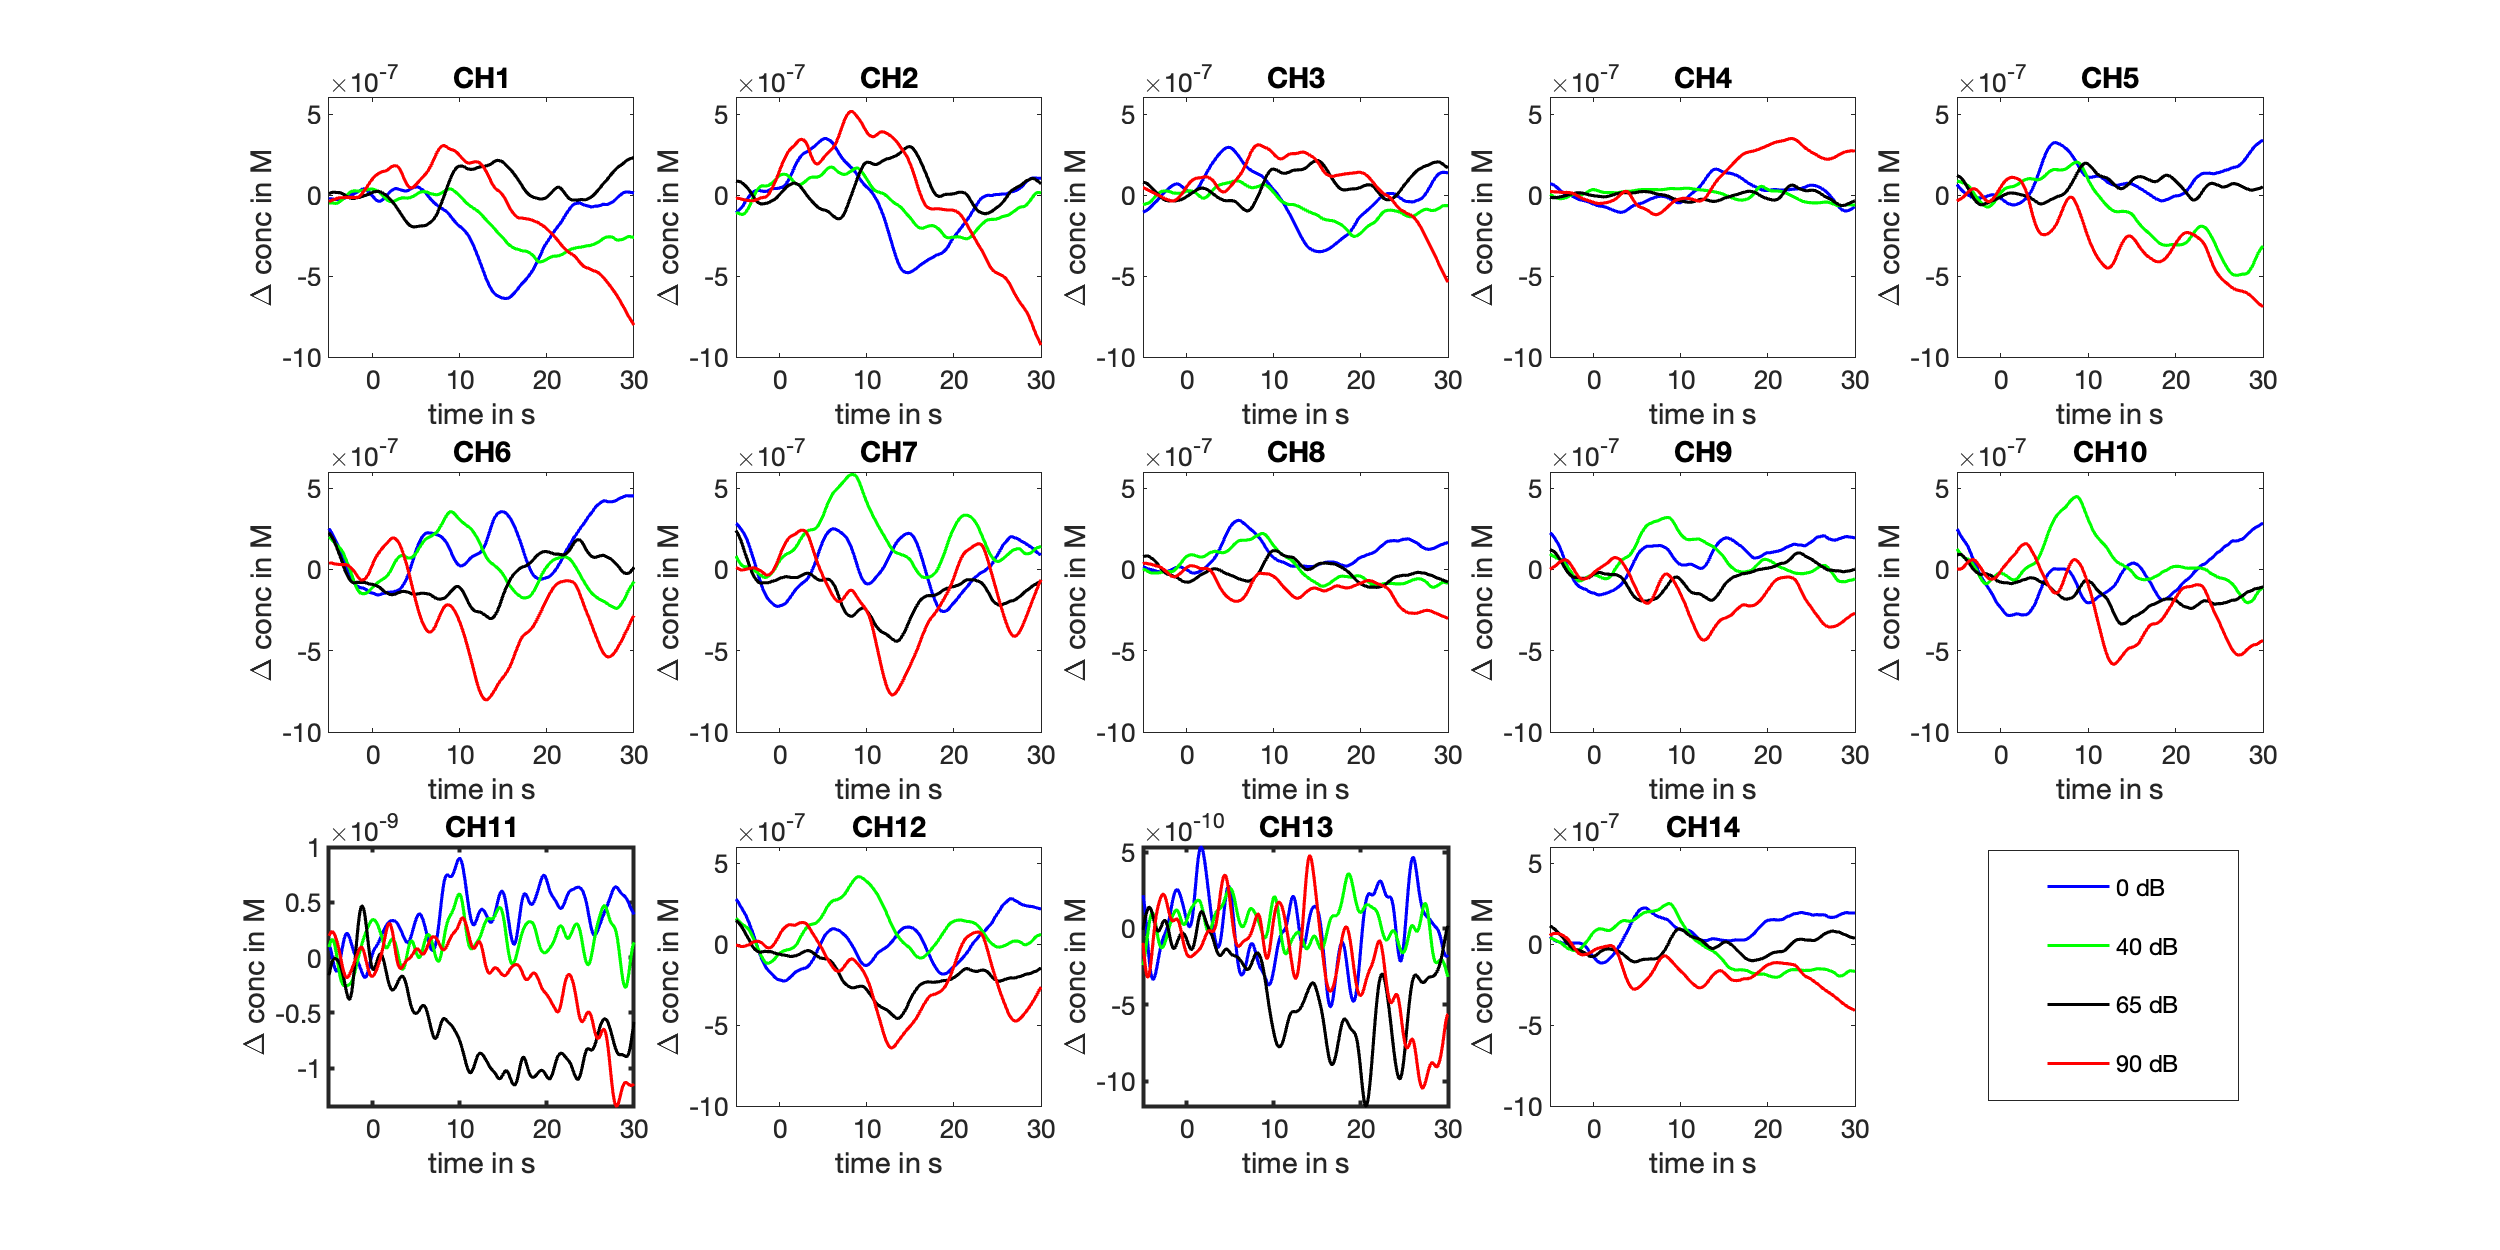
\includegraphics[scale=.4]{bilder/HbO_Mole/sub_gleb2_s_HbO.png}
  \caption{HbO measurement from participant 2.}
  \label{fig:somesignal}
  \medskip
  \footnotesize {Lines represent the block-averaged results over eight epochs. The averaged change of HbO concentration (in Mole) is plotted from 5 seconds before the start of the auditory stimuli to 30 seconds after the start of the stimuli. Four colours are used to differentiate the response from sound stimuli of different intensity levels.}
\end{figure}

\newpage

\begin{figure}[H]
  \centering
    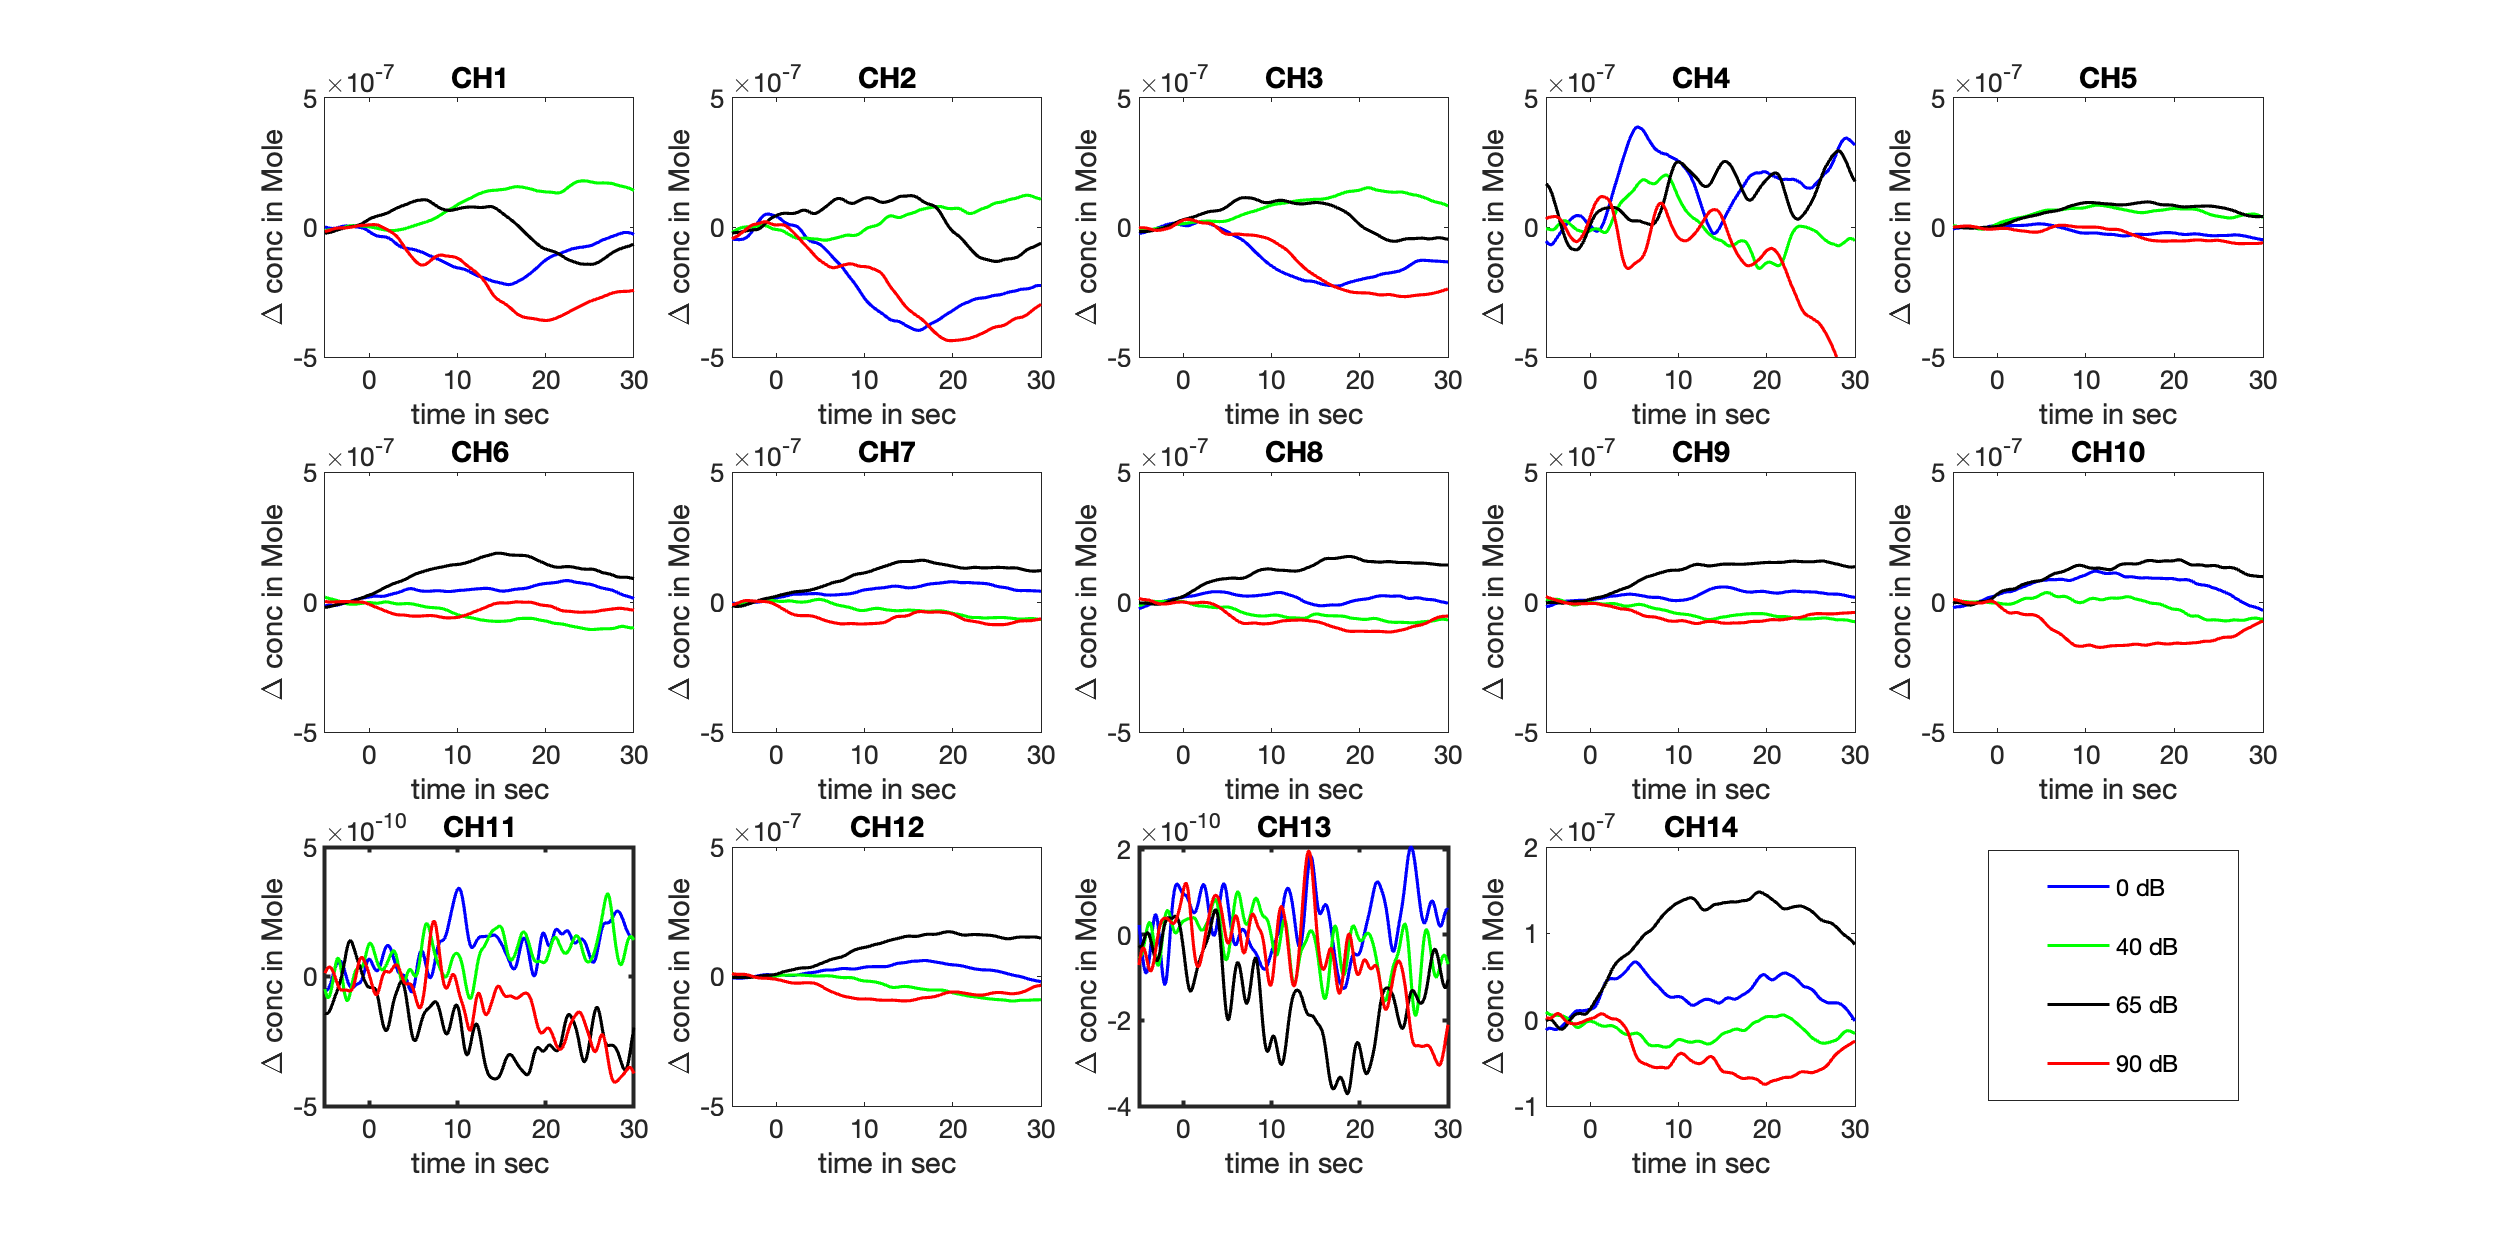
\includegraphics[scale=.4]{bilder/HbR_Mole/sub_gleb2_s_HbR.png}
  \caption{HbR measurement from participant 2.}
  \label{fig:somesignal}
  \medskip
  \footnotesize {Lines represent the block-averaged results over eight epochs. The averaged change of HbR concentration (in Mole) is plotted from 5 seconds before the start of the auditory stimuli to 30 seconds after the start of the stimuli. Four colours are used to differentiate the response from sound stimuli of different intensity levels.}
\end{figure}

\begin{figure}[H]
  \centering
    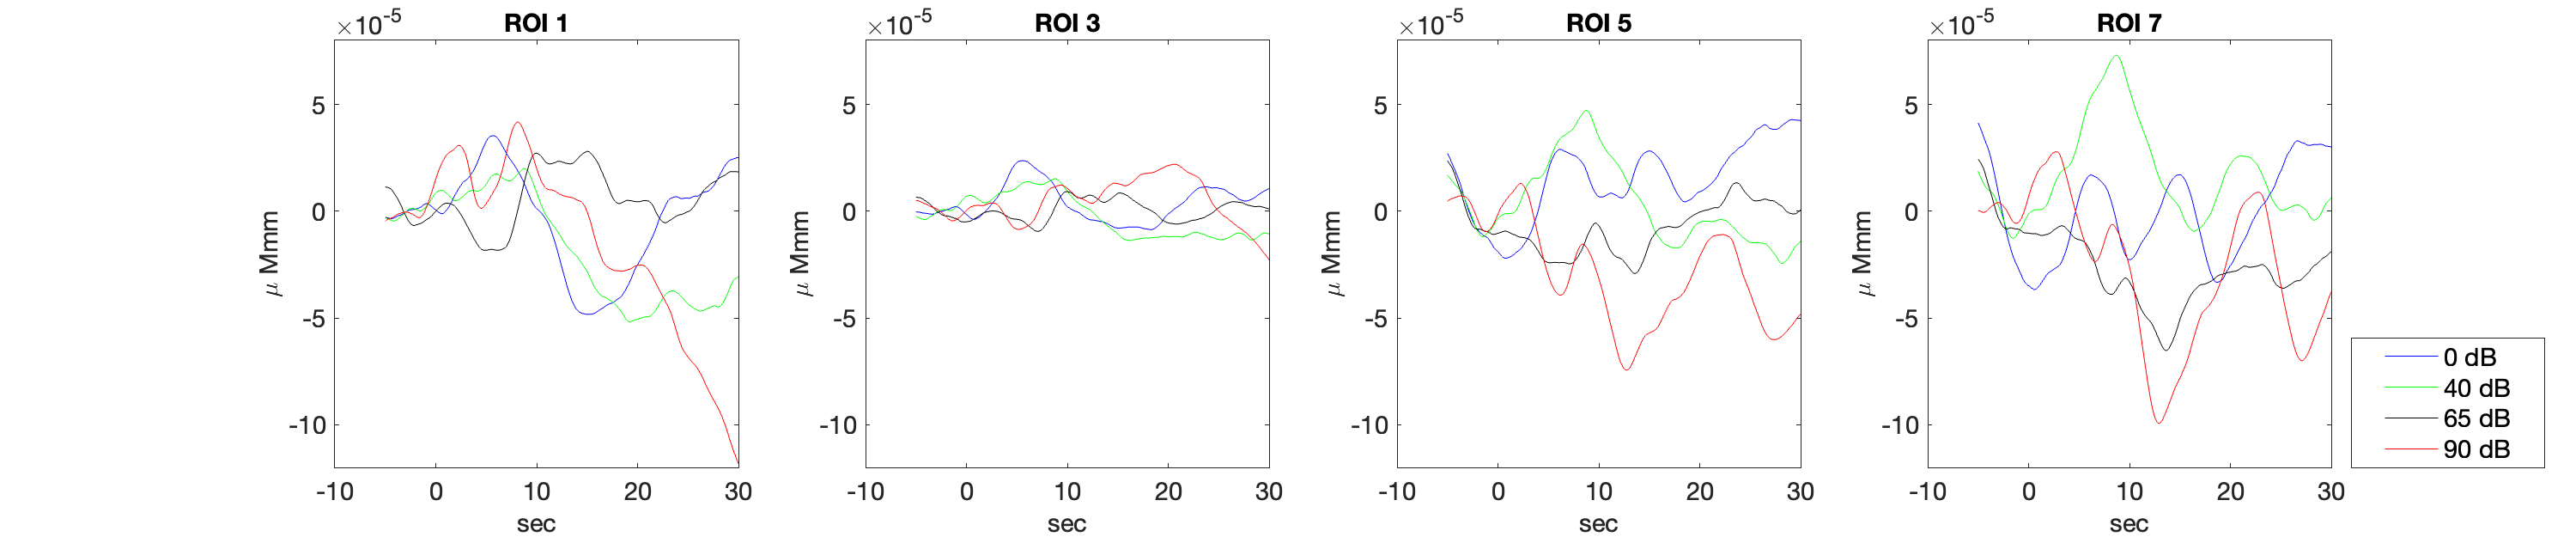
\includegraphics[scale=.29]{bilder/ROI/sub_gleb2_s_HbO.png}
  \caption{ROI measurement from participant 2.}
\end{figure}

\newpage

\section {Participant 6}
\begin{figure}[H]
  \centering
    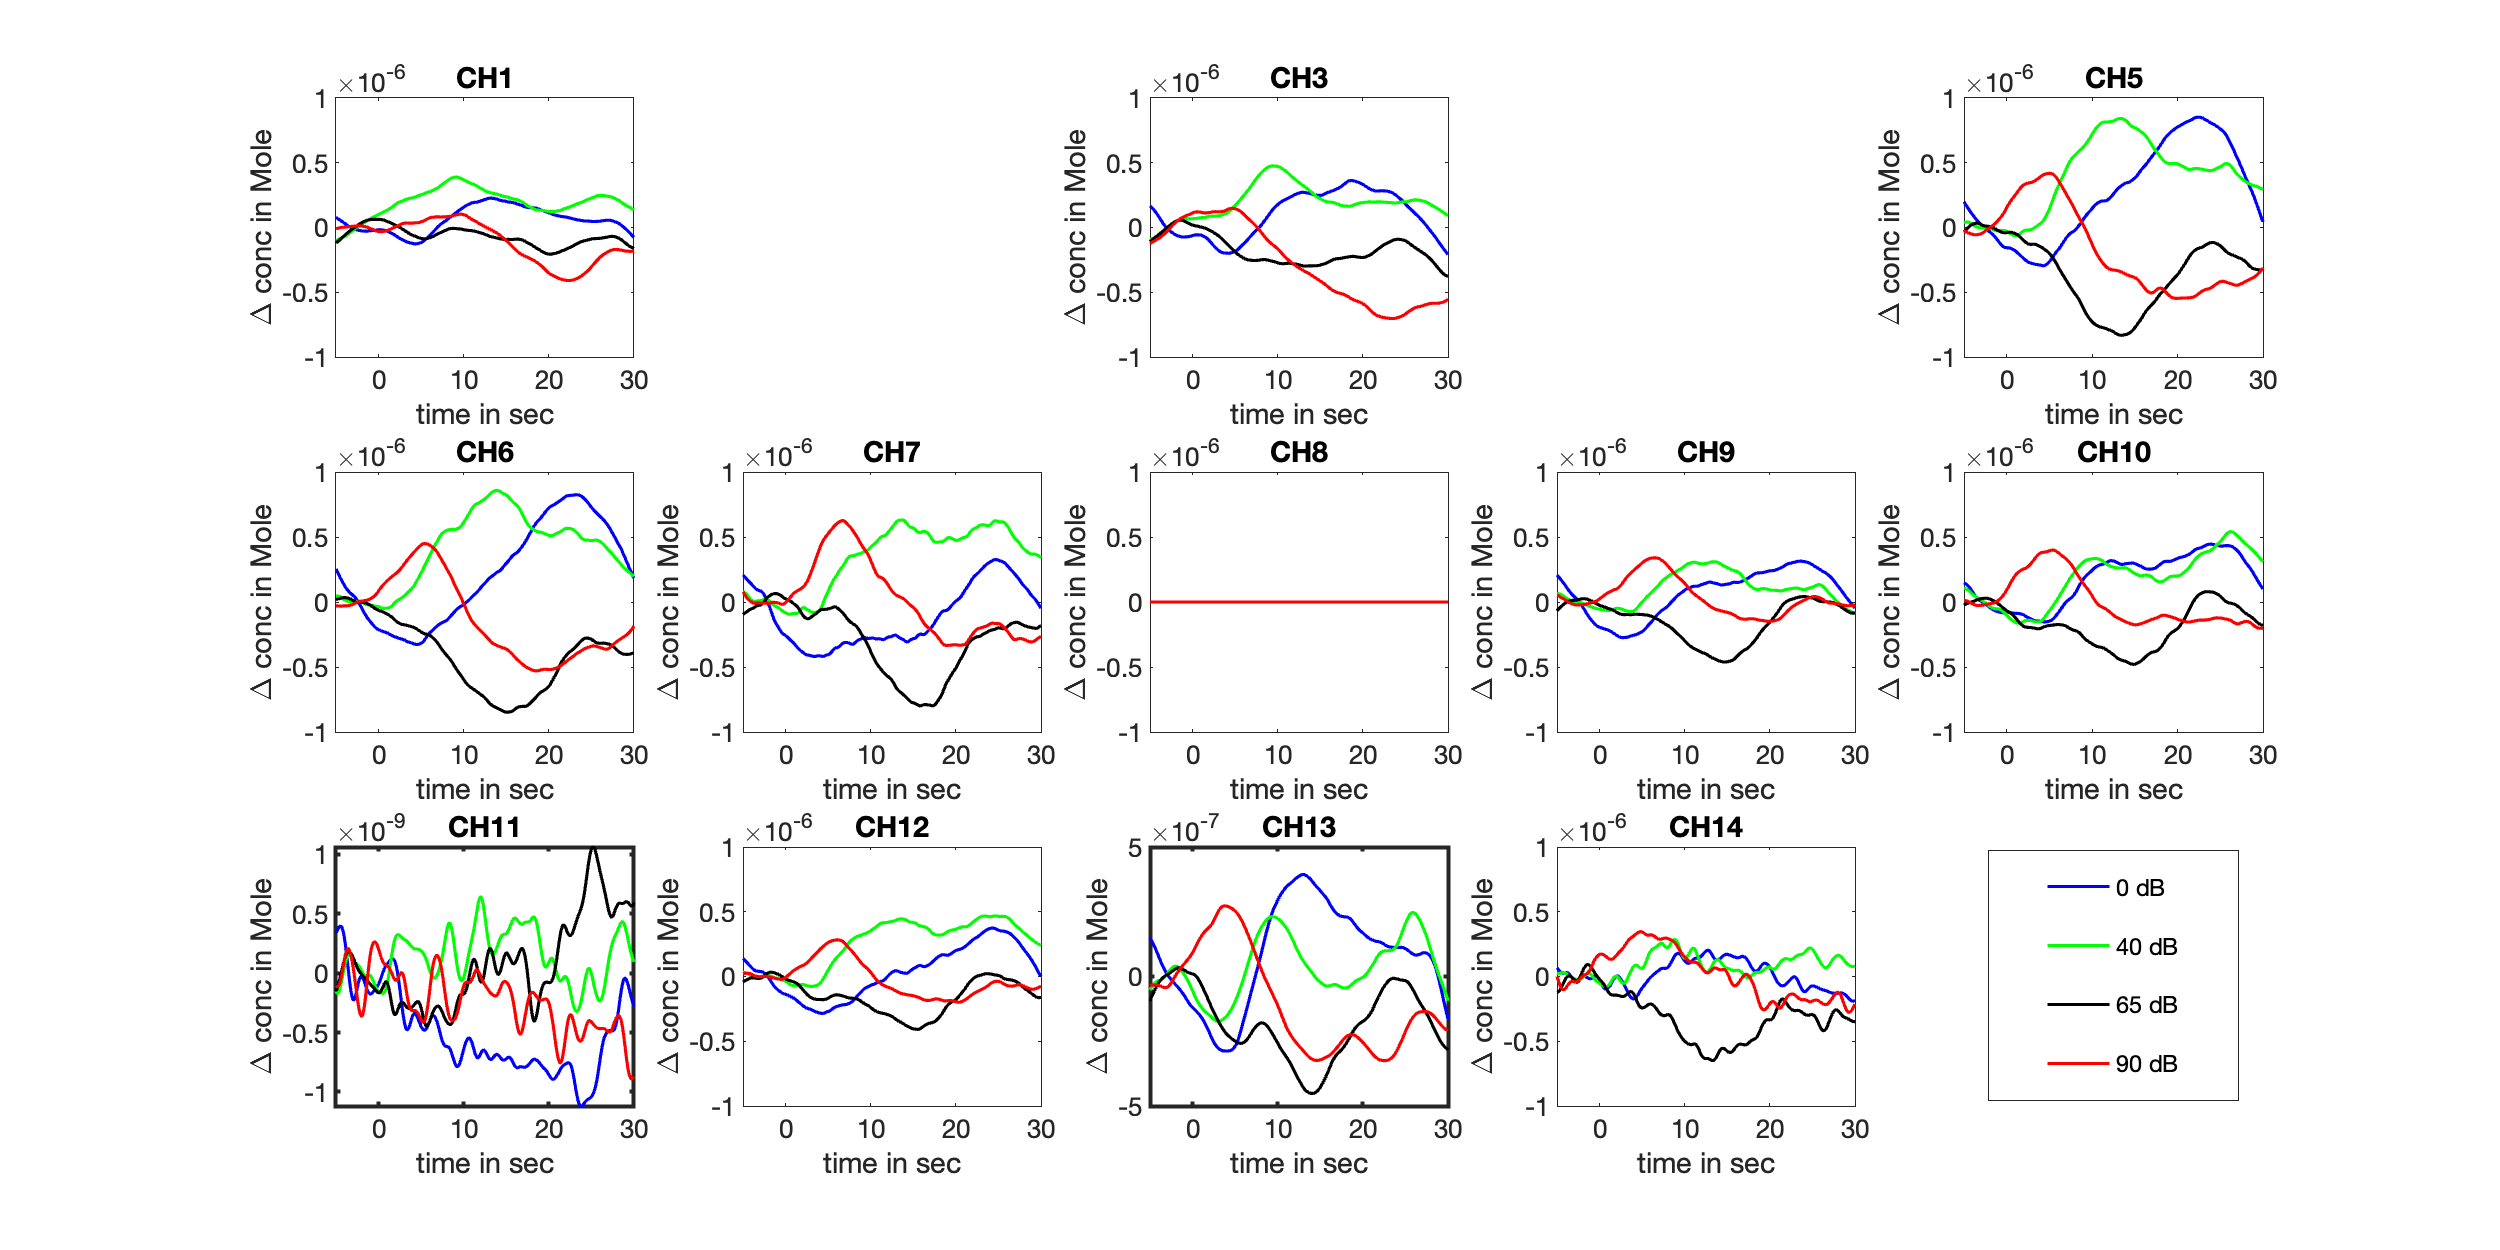
\includegraphics[scale=.4]{bilder/HbO_Mole/sub_shelia_s_HbO.png}
  \caption{HbO Measurement from participant 6.}
  \label{fig:somesignal}
  \medskip
  \footnotesize {Lines represent the block-averaged results over eight epochs. The averaged change of HbO concentration (in Mole) is plotted from 5 seconds before the start of the auditory stimuli to 30 seconds after the start of the stimuli. Four colours are used to differentiate the response from sound stimuli of different intensity levels.}
\end{figure}


\newpage


\begin{figure}[H]
  \centering
    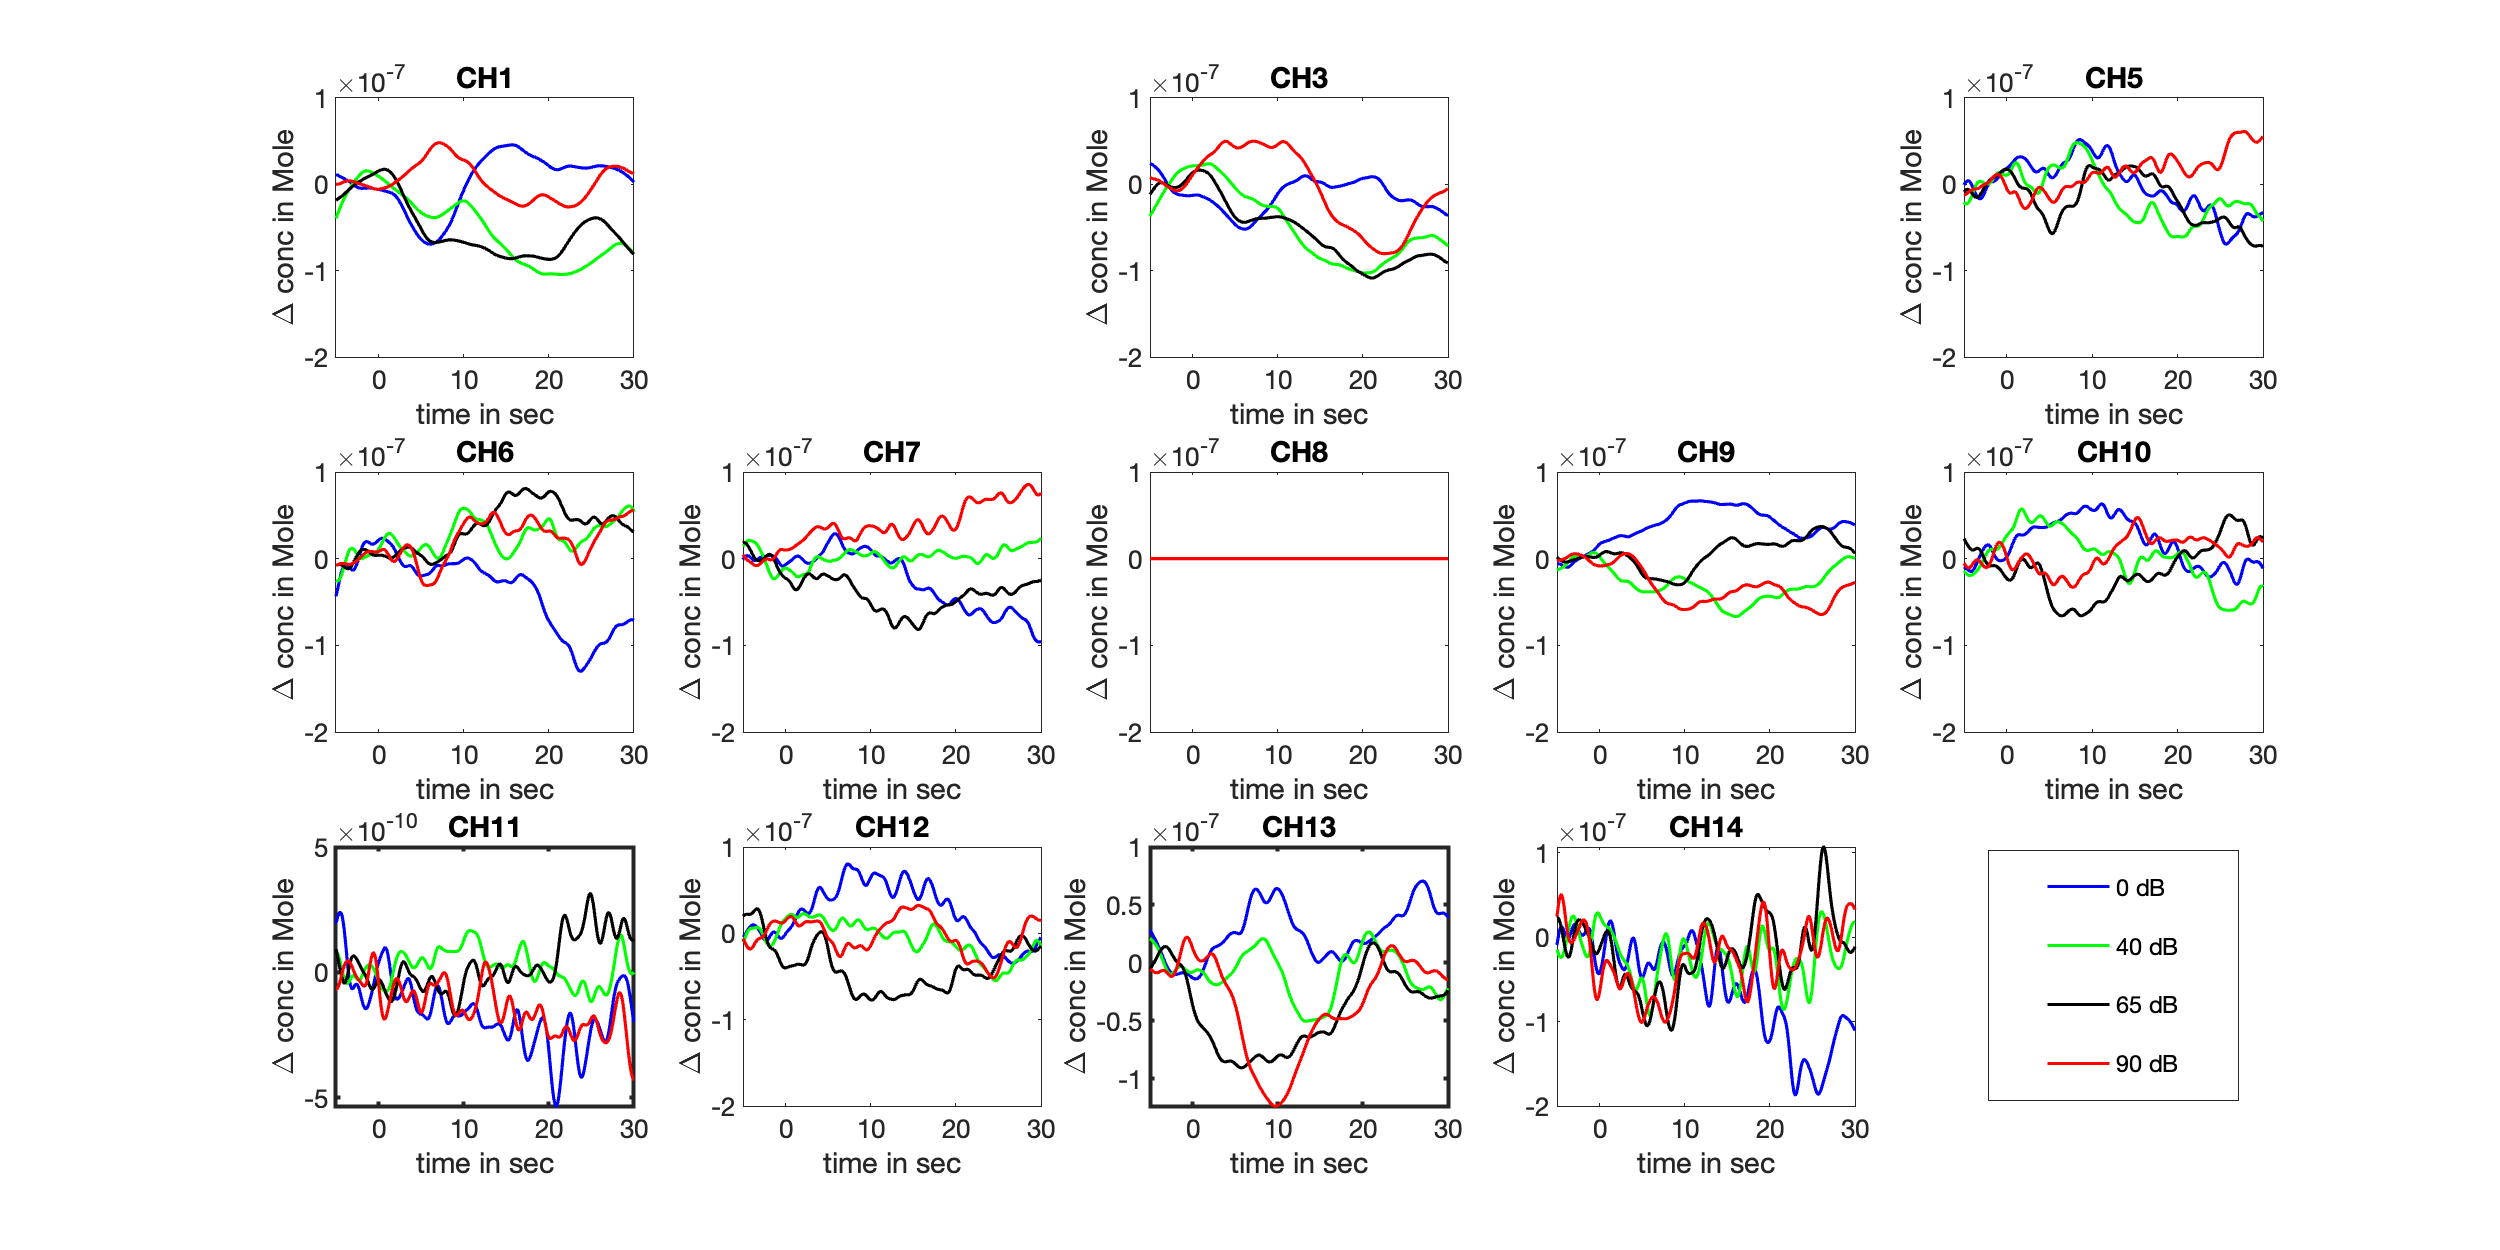
\includegraphics[scale=.4]{bilder/HbR_Mole/sub_shelia_s_HbR.png}
  \caption{HbR Measurement from participant 6.}
  \label{fig:somesignal}
  \medskip
  \footnotesize {Lines represent the block-averaged results over eight epochs. The averaged change of HbR concentration (in Mole) is plotted from 5 seconds before the start of the auditory stimuli to 30 seconds after the start of the stimuli. Four colours are used to differentiate the response from sound stimuli of different intensity levels.}
\end{figure}

\begin{figure}[H]
  \centering
    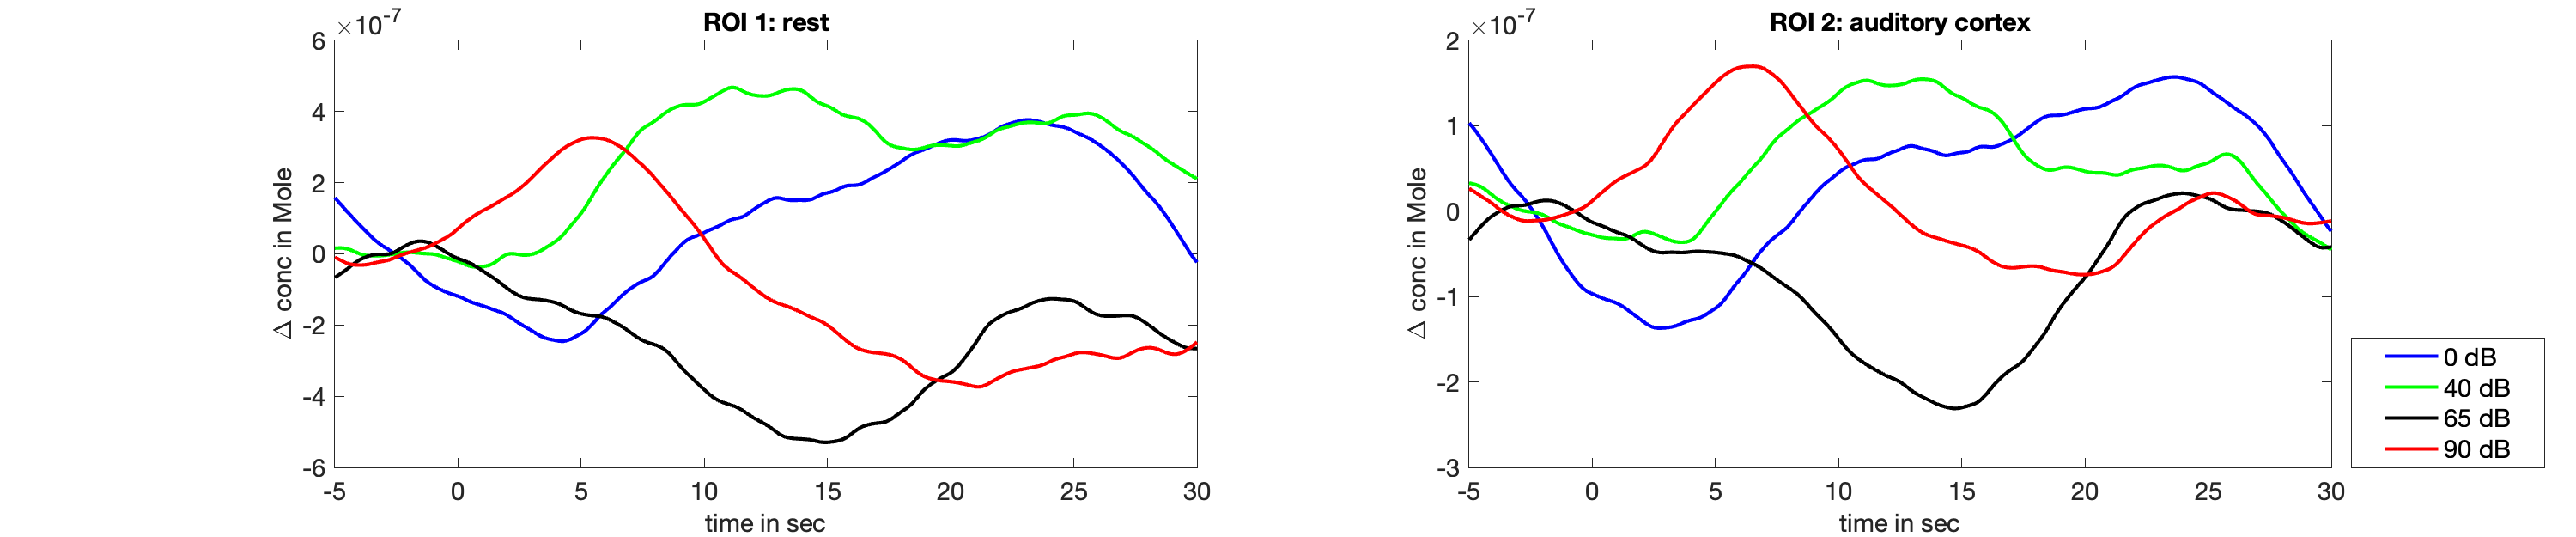
\includegraphics[scale=.29]{bilder/ROI/sub_shelia_s_HbO.png}
  \caption{ROI Measurement from participant  6.}
\end{figure}

For the oxygenated hemoglobin, \acrshort{HbO} waveform, the loudest sound stimuli resulted in phasic response for almost all the channels. In addition, it also resulted in faster on-set compared with other stimuli of lower sound pressure levels.

On the other hand, as for the deoxygenated hemoglobin, \acrshort{HbR} response, results from multiple channels appeared to be noisy even if the SCI values were already above the suggested threshold.

\newpage

\section {Participant 8}

\begin{figure}[H]
  \centering
    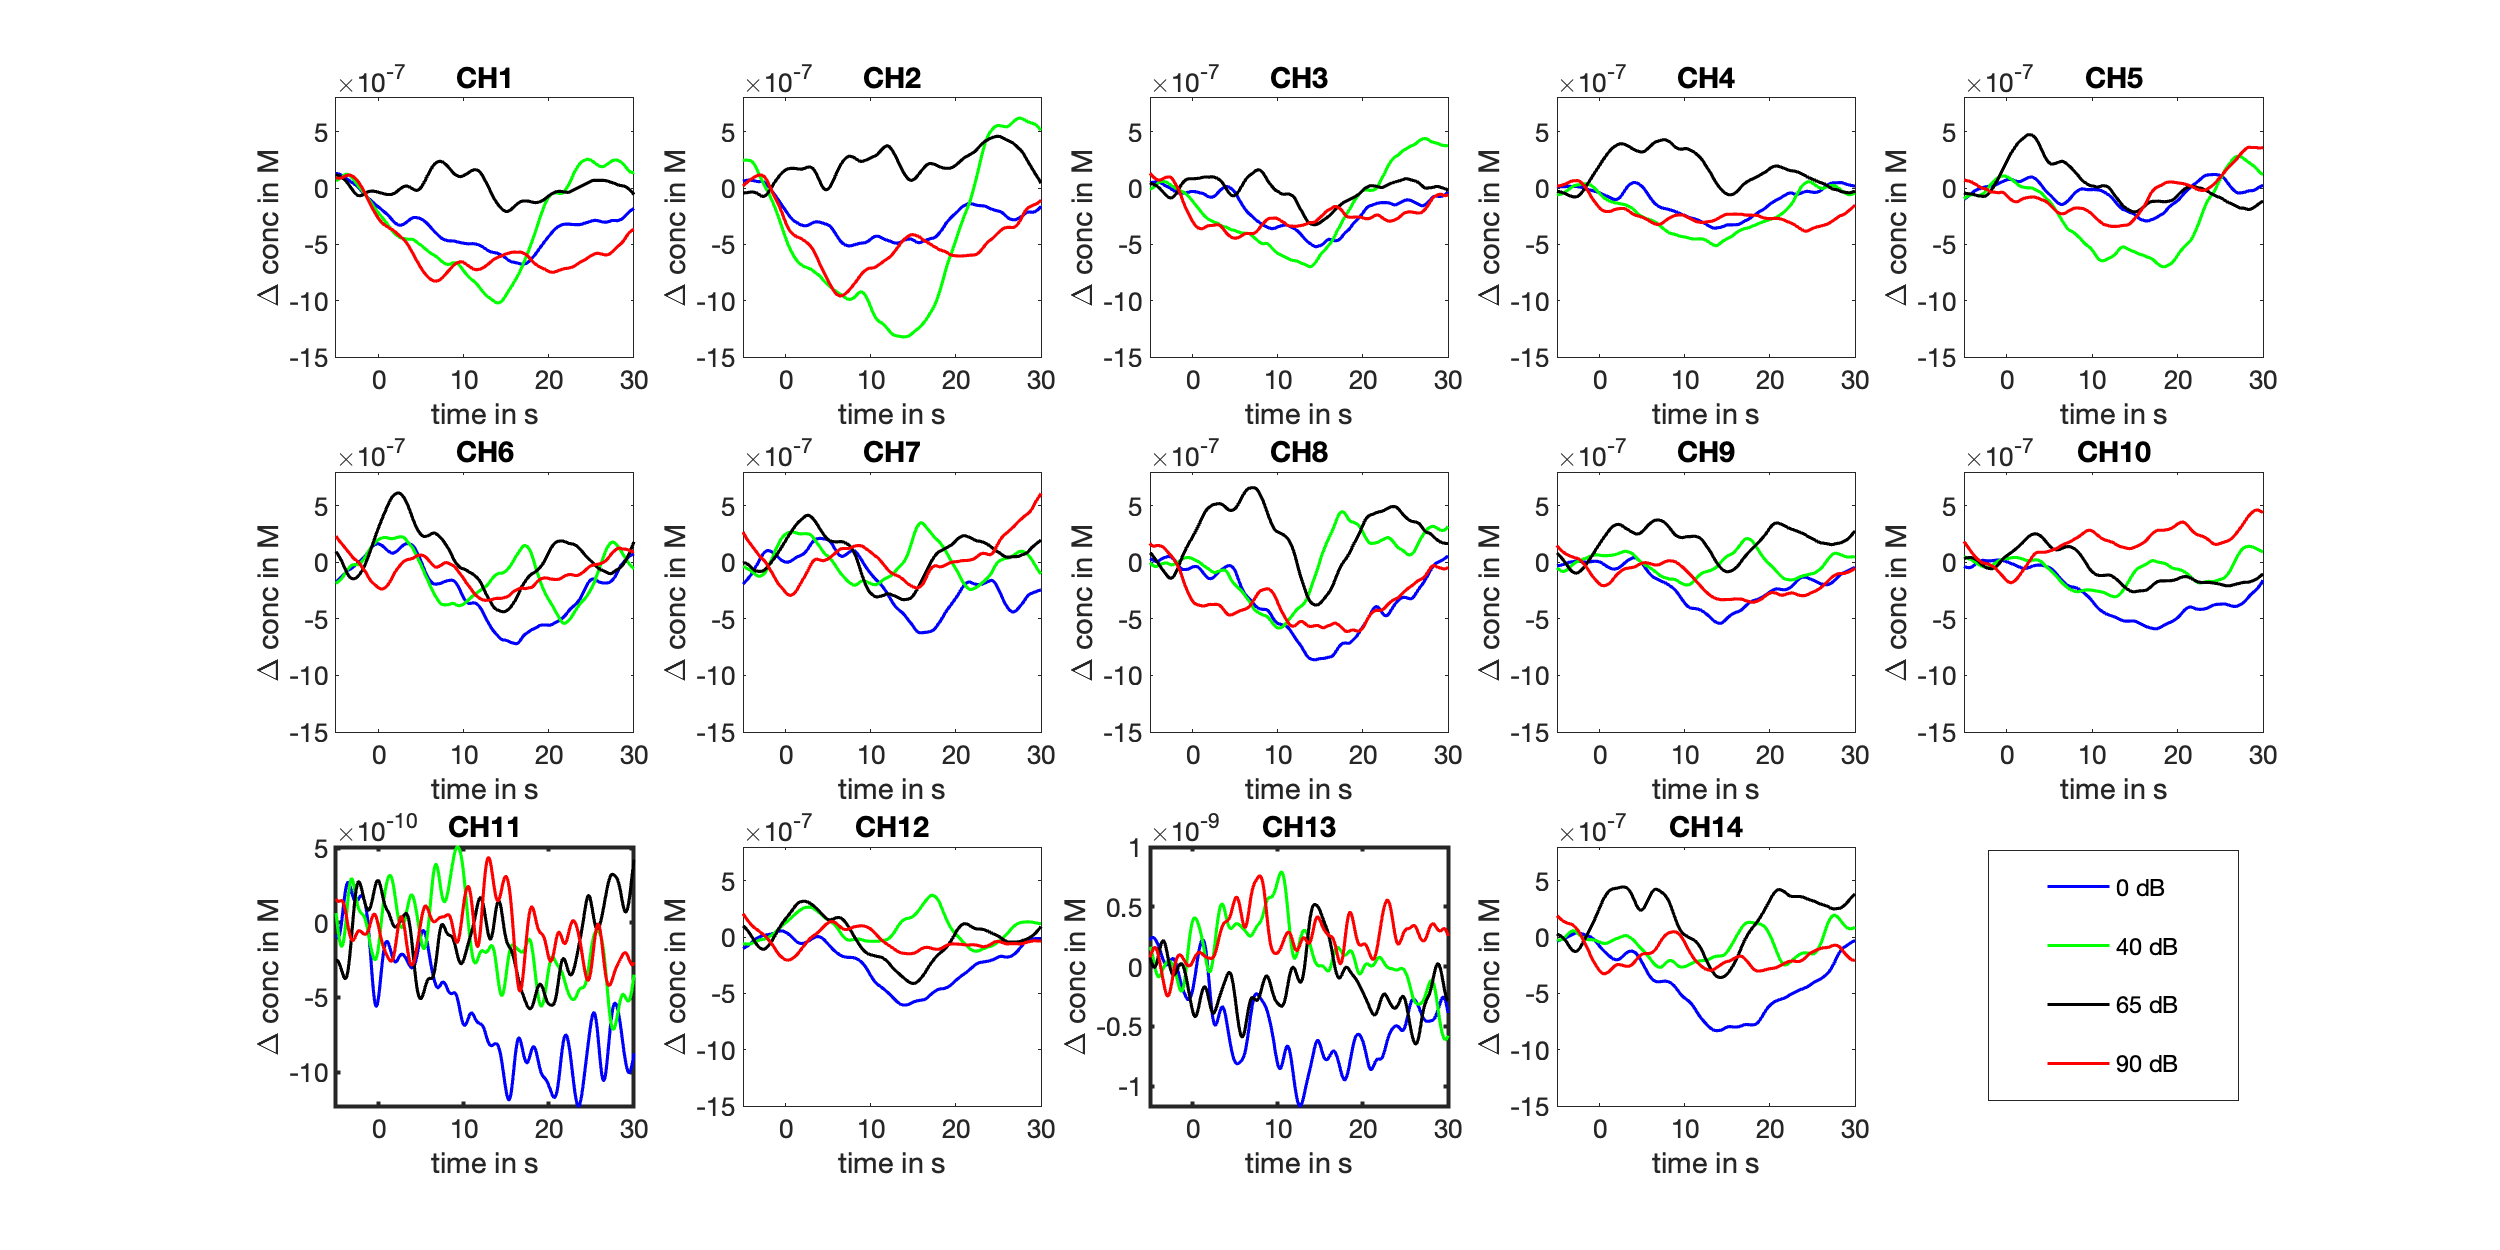
\includegraphics[scale=.4]{bilder/HbO_Mole/sub_luca2_s_HbO.png}
  \caption{HbO measurement from participant 8. Silent comparison}
  \label{fig:somesignal}
  \medskip
  \footnotesize {Lines represent the block-averaged results over eight epochs. The averaged change of HbO concentration (in Mole) is plotted from 5 seconds before the start of the auditory stimuli to 30 seconds after the start of the stimuli.}
\end{figure}

\newpage

\begin{figure}[H]
  \centering
    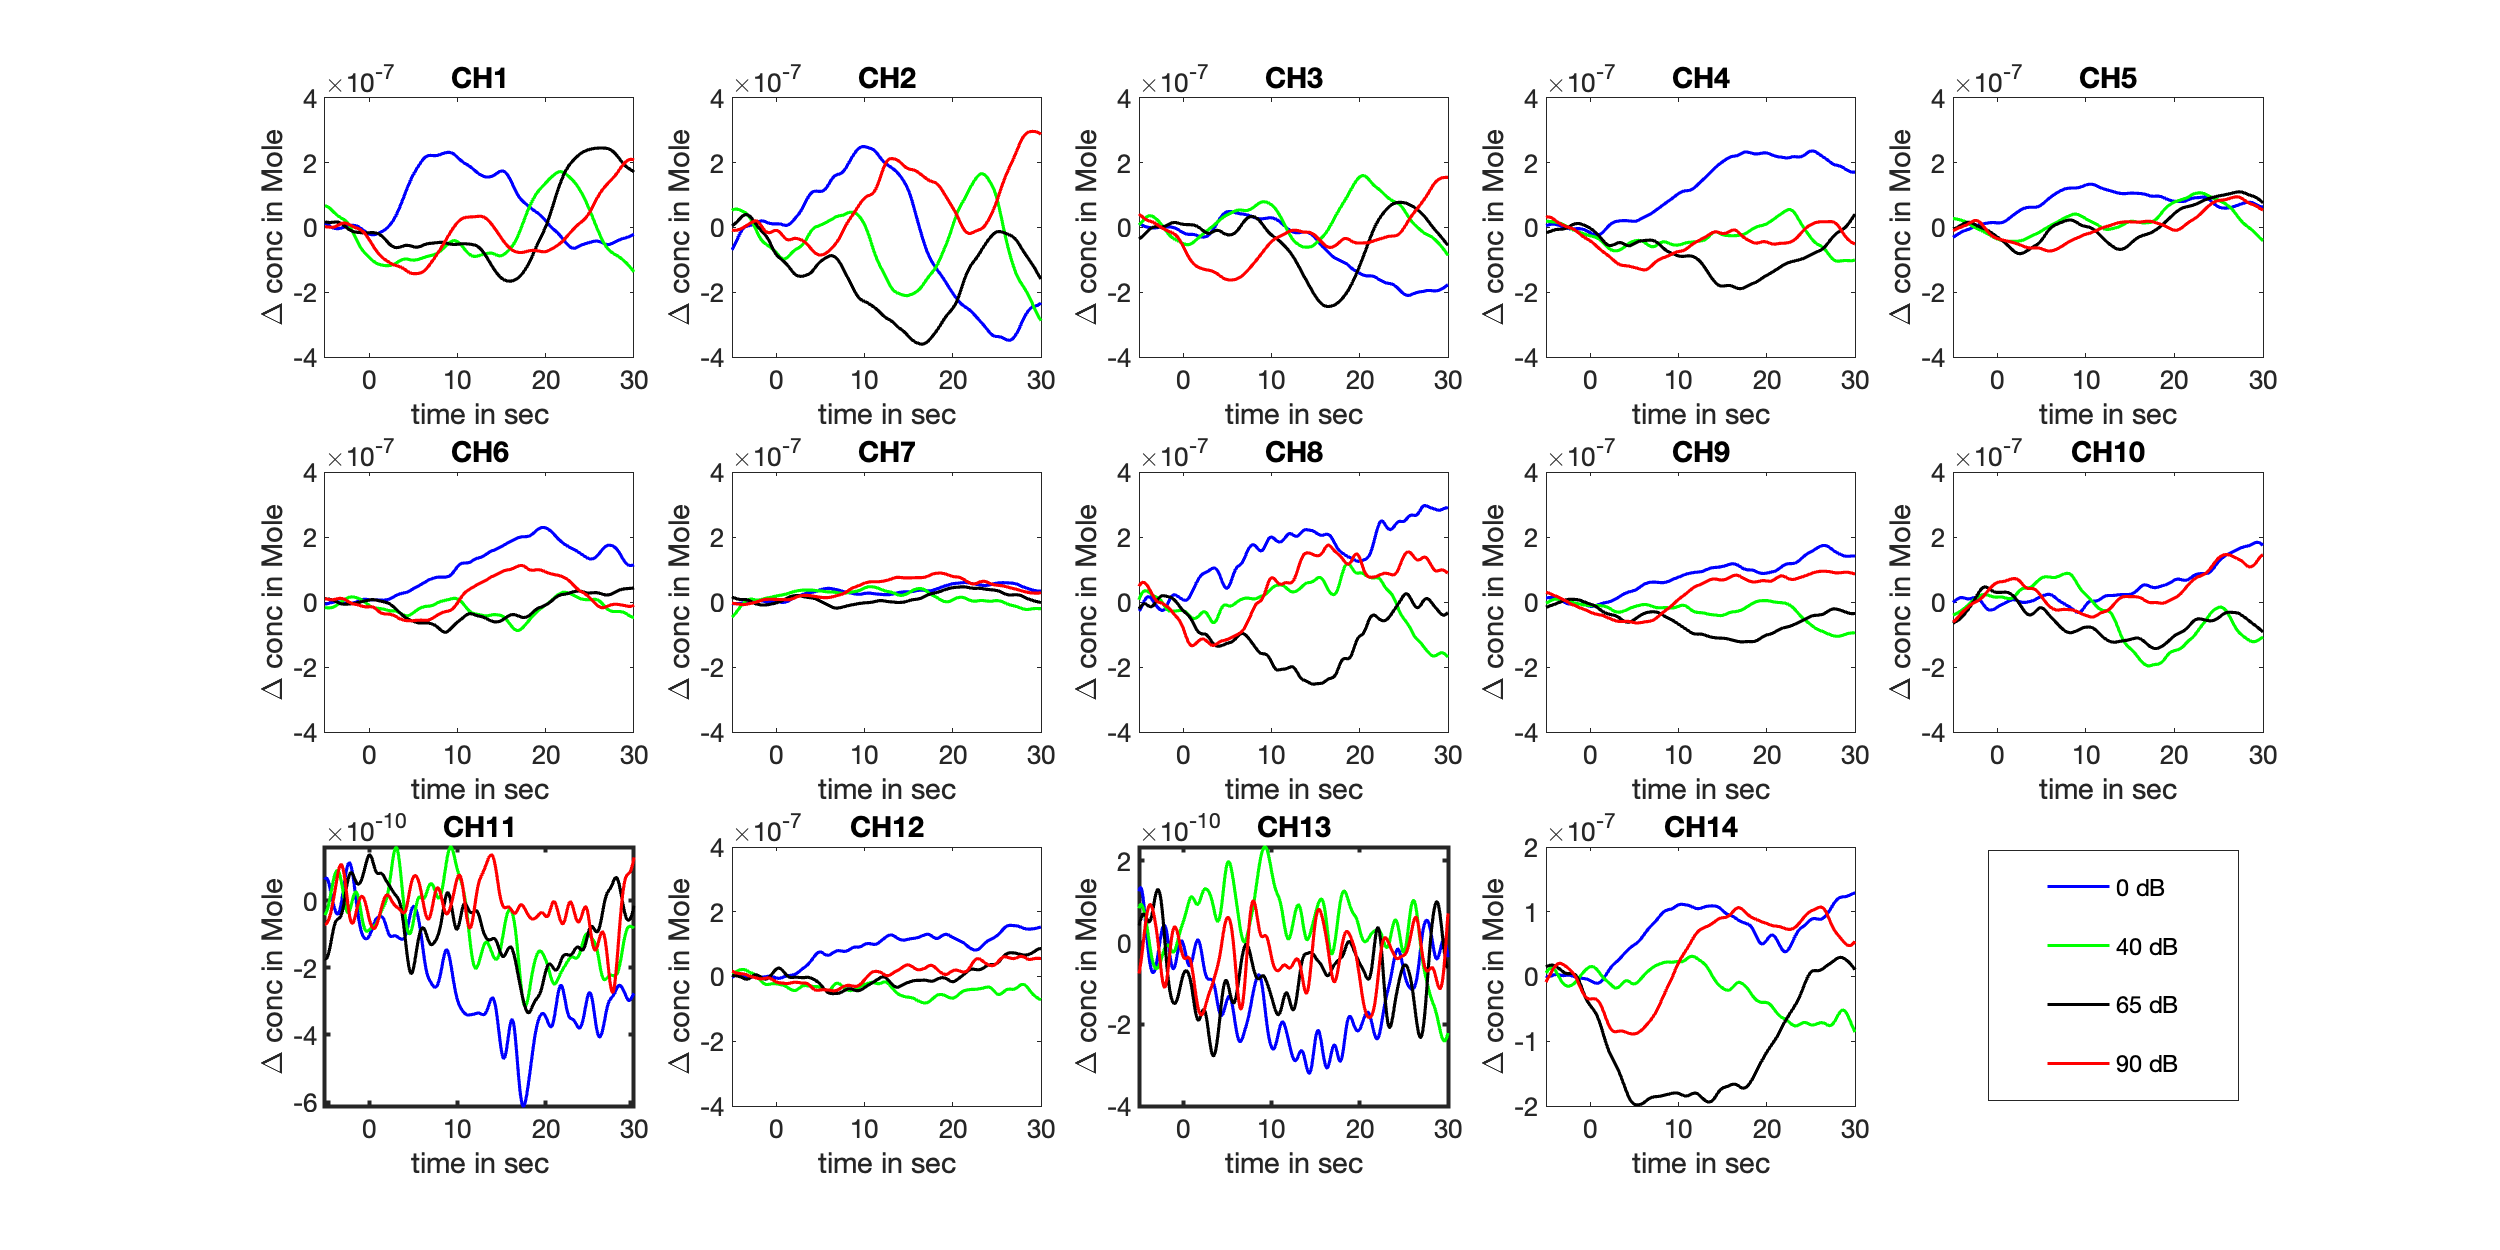
\includegraphics[scale=.4]{bilder/HbR_Mole/sub_luca2_s_HbR.png}
  \caption{HbR measurement from participant 8. Silent comparison}
  \medskip
  \footnotesize {Lines represent the block-averaged results over eight epochs. The averaged change of HbR concentration (in Mole) is plotted from 5 seconds before the start of the auditory stimuli to 30 seconds after the start of the stimuli.}
\end{figure}

\begin{figure}[H]
  \centering
    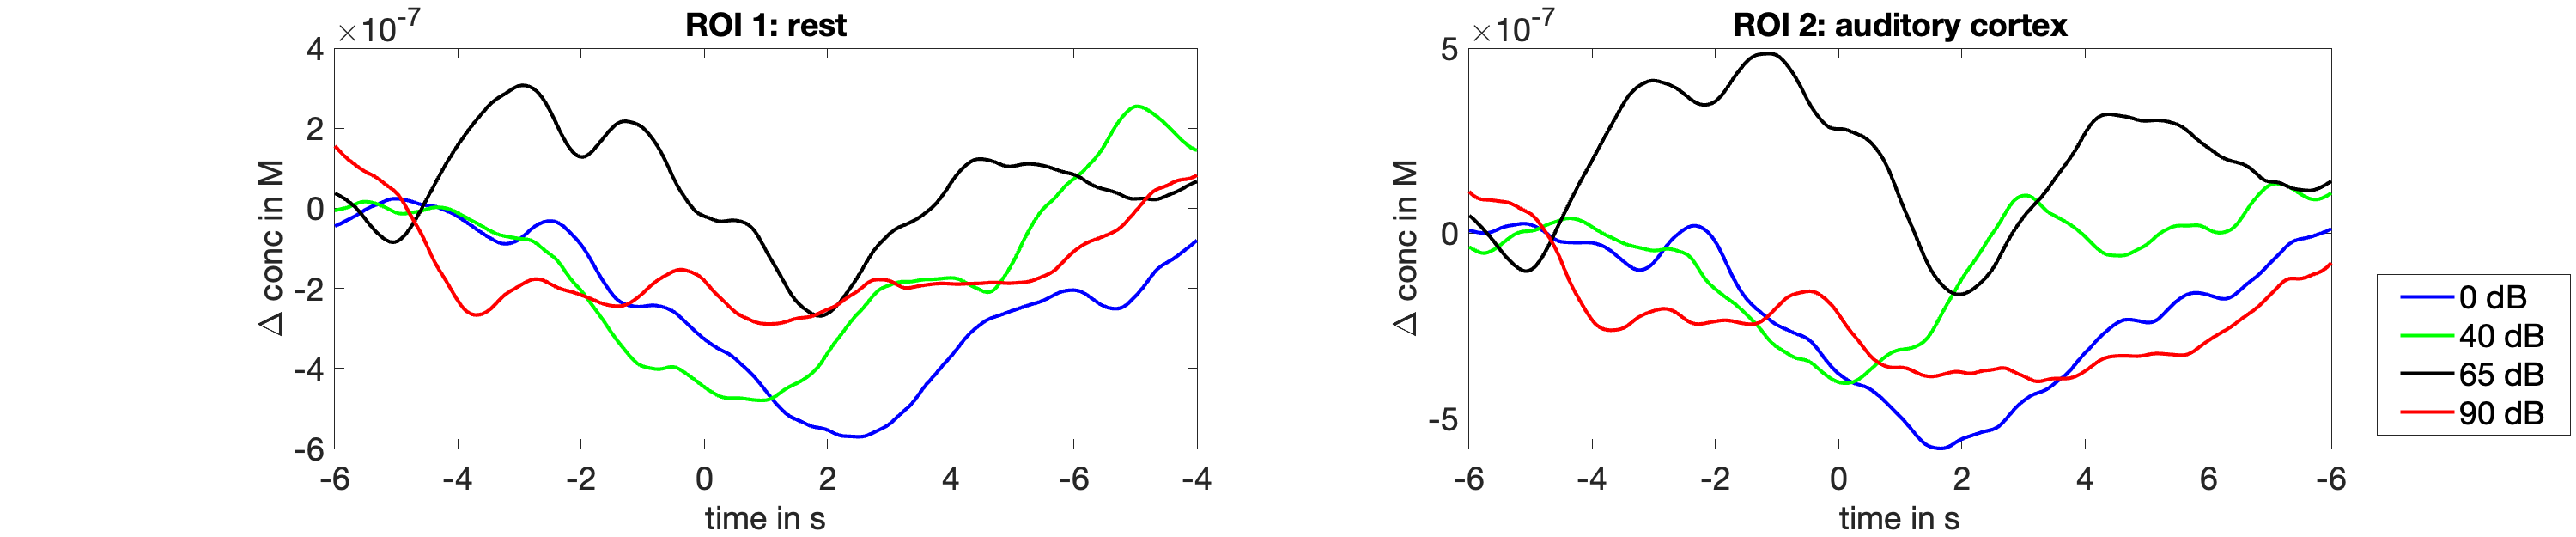
\includegraphics[scale=.29]{bilder/ROI/sub_luca2_s_HbO.png}
  \caption{ROI measurement from participant 8. Silent comparision.}
\end{figure}

This participant was given only silence stimuli. No pattern could be concluded for the measured waveform morphology. Nonetheless, it is noteworthy to know that even if there were almost no visual and sound stimuli, dynamic hemoglobin response still presented.